\chapter{ID stage}
\label{chap:id}

In the ID stage instructions are decoded and the register file is accessed. Its block diagram is shown in picture \ref{fig:ID_stage}

\begin{figure}[!ht]
	\centering
	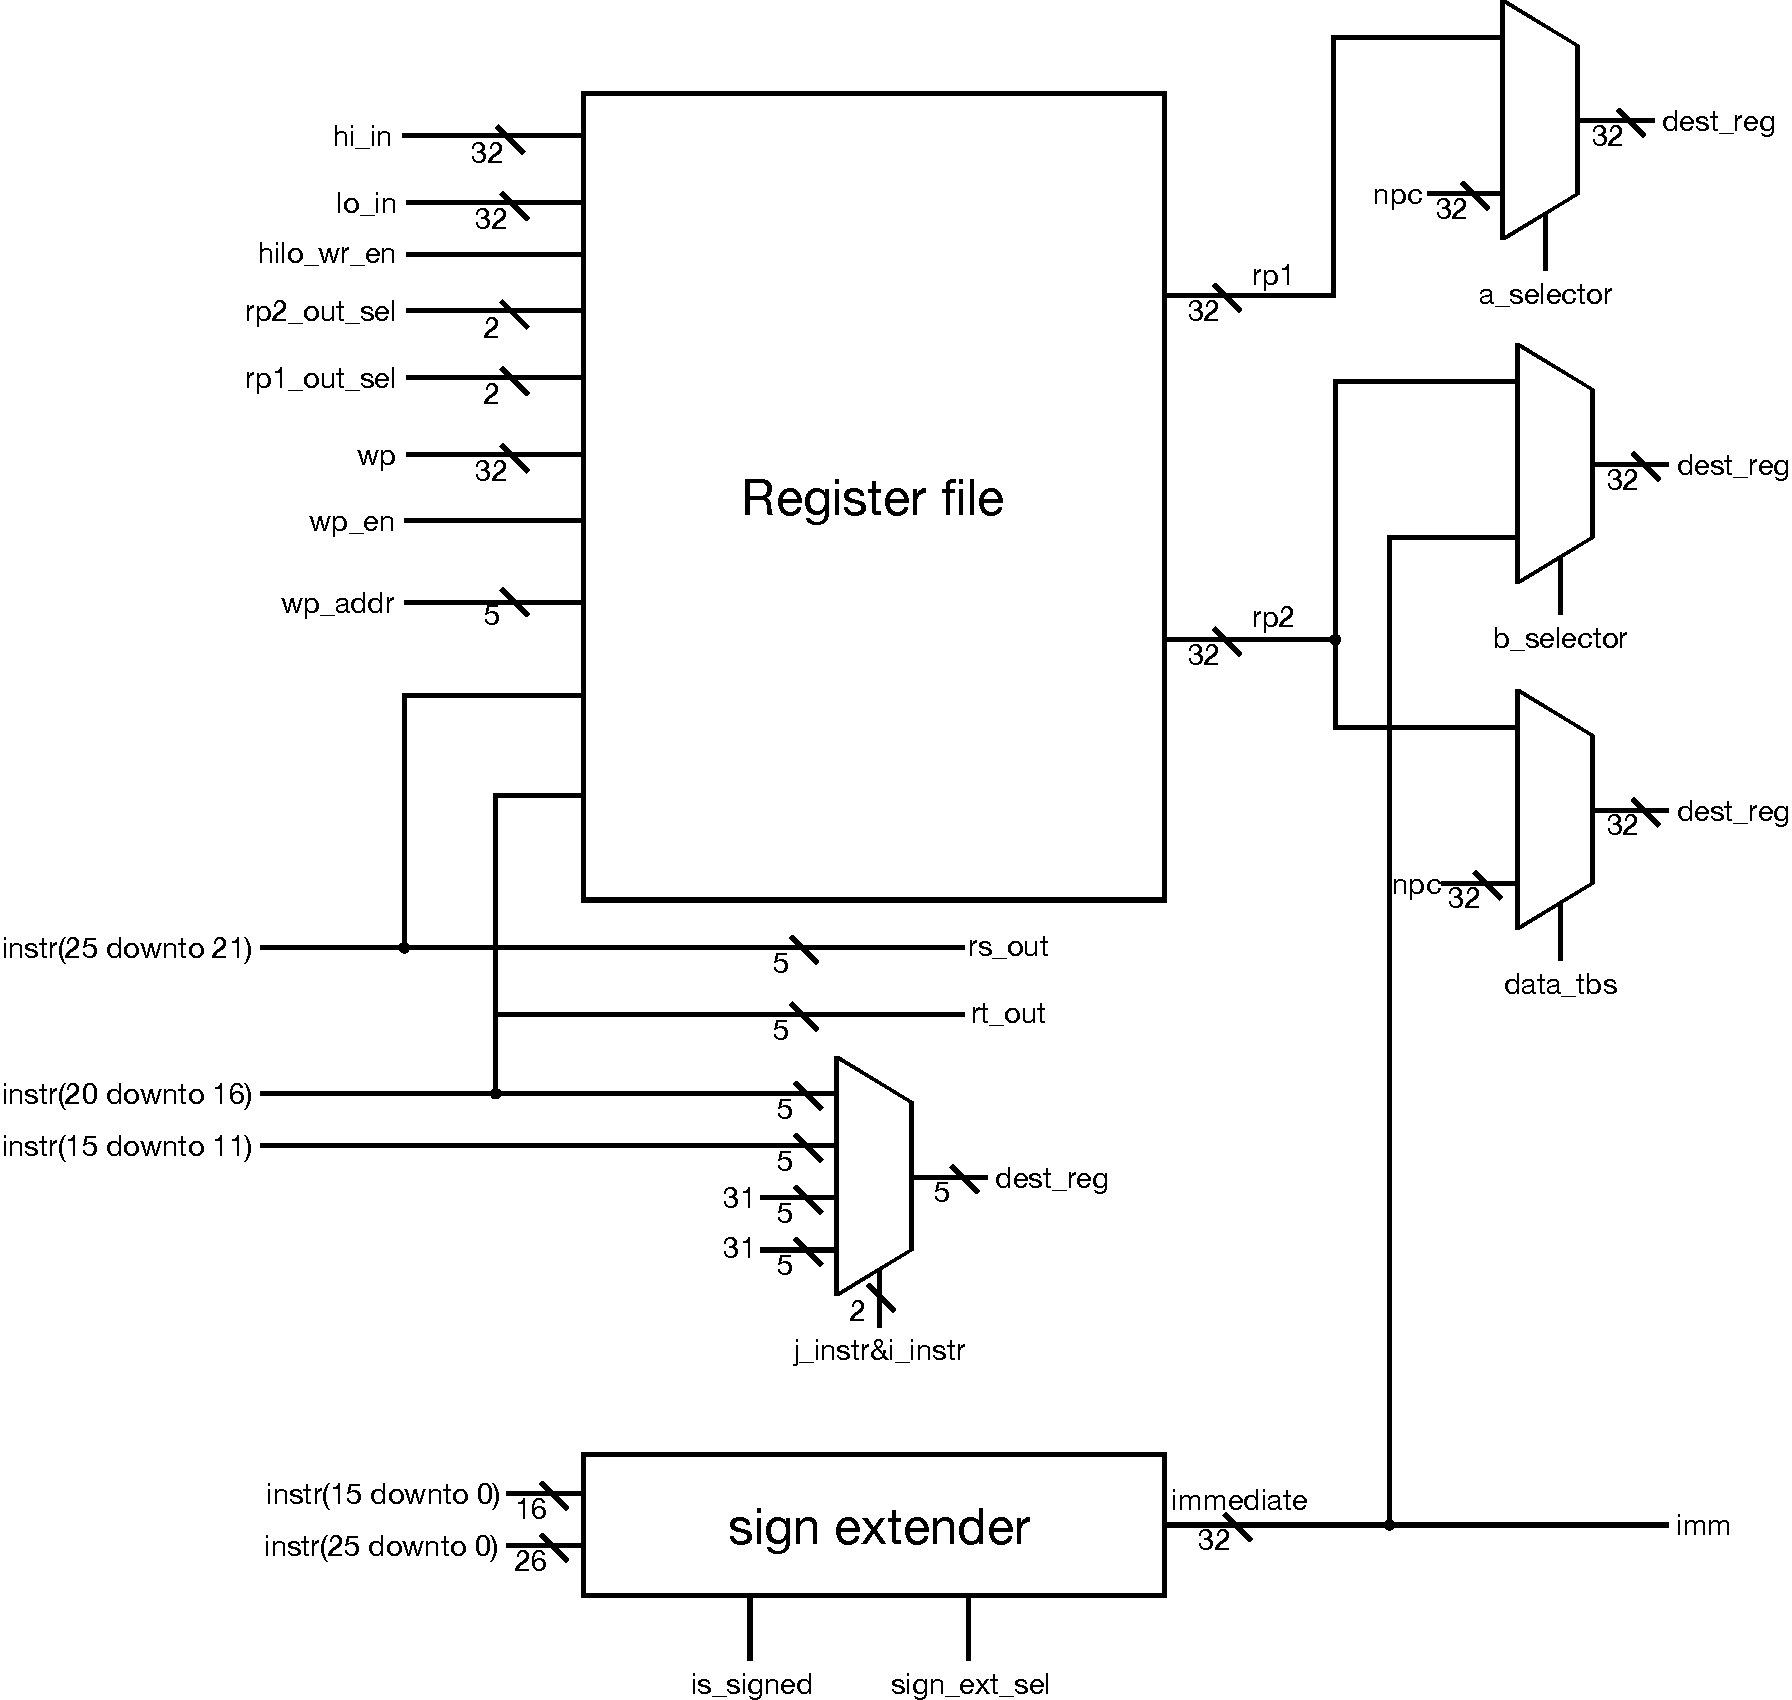
\includegraphics[width=.6\linewidth]{./chapters/figures/ID_stage.pdf}
	\caption{Block diagram of the ID stage}
	\label{fig:ID_stage}
\end{figure}

\section{Register file}

The {\it register file} is one of the two main components in this stage. It has 2 read ports and 3 write ports, although a write operation never use all of them at the same time.
It contains 32 {\it general purpose registers} (GPR), as stated by the ABI, and 2 additional registers called \verb|lo| and \verb|hi|, accessible only by special instructions and used
to store multiplications' results. Among the GPR there is a special register, the register number 0, that cannot be written and always contains the value \verb|0x00000000|.
The full list of the ABI-compliant registers is shown in table \ref{tab:registers}:

\begin{table}[!ht]
    \centering
    \begin{tabular}{ |c|c|c|c| }
        \hline
        Name & Number & Use & Directly accessible \\

        \hline
        \verb|$zero| & 0 & constant 0 & Yes \\
        \hline
        \verb|$at| & 1 & assembler temporary & Yes \\
        \hline
        \verb|$v0-$v1| & 2-3 & values for function returns and expression evaluation & Yes \\
        \hline
        \verb|$a0-$a3| & 4-7 & function arguments & Yes \\
        \hline
        \verb|$t0-$t7| & 8-15 & temporaries & Yes \\
        \hline
        \verb|$s0-$s7| & 16-23 & saved temporaries & Yes \\
        \hline
        \verb|$t8-$t9| & 24-25 & temporaries & Yes \\
        \hline
        \verb|$k0-$k1| & 26-27 & reserved for OS kernel & Yes \\
        \hline
        \verb|$gp| & 28 & global pointer & Yes \\
        \hline
        \verb|$sp| & 29 & stack pointer & Yes \\
        \hline
        \verb|fp| & 30 & frame pointer & Yes \\
        \hline
        \verb|$ra| & 31 & return address & Yes \\
        \hline
        \verb|$lo| & 32 & stores the lower 32 bits of a multiplication & No \\
        \hline
        \verb|$hi| & 33 & stores the higher 32 bits of a multiplication & No \\
        \hline
    \end{tabular}
    \caption{DLX registers. Taken from \cite{abi_regs}}
    \label{tab:registers}
\end{table}

In the ID stage the RF is accessed in read, since it is the WB stage to access it in write. To select the registers the bits 25-21 and 20-11 are used,
because they represent the \verb|rs| and \verb|rt| fields in an R instruction. These values are not the only ones used by the RF to decide which values
its read ports should take: as illustrated in table \ref{tab:registers}, there are two non-directly accessible registers, \verb|lo| and \verb|hi|. To perform
the final output selection two control signals are used, \verb|rp1_out_sel| and \verb|rp2_out_sel|, that drive 2 internal muxes that choose the value of the read ports as follows:

\begin{enumerate}
    \item \verb|00|: output the selected GP register.
    \item \verb|01|: output the \verb|lo| register.
    \item \verb|10|: output the \verb|hi| register.
    \item \verb|11|: output \verb|0x00000000|.
\end{enumerate}

\section{Sign extender}

This component is used by I and J instructions to extend their immediate fields on 32 bits. In fact, I instructions have their immediate stored in the lower 16 bits of the instruction,
while the J have it stored on the lower 26 bits. Moreover, these bits could represent a signed or unsigned value, like in the case of a \verb|addi| and a \verb|addui|, therefore this
has to be taken in account during the extension. As shown in figure \ref{fig:ID_stage}, two controls signals enter the sign extender: \verb|is_signed| and \verb|sign_ext_sel|. The former
is used to extend either with 0s or taking into account the sign, while the latter is used to decide if the extension should consider only 16 bits or 26.

\section{Selection muxes}

In the rightmost part of figure \ref{fig:ID_stage} 3 muxes 2x1 can be seen. In a standard MIPS pipeline these would reside in the EXE stage, but since it is the slowest stage of the pipeline
we decided to shorten its critical path by bringing them in the ID stage. The first mux is used to select between the read port 1 of the RF and the program counter coming from the stage before,
while the second mux chooses among the RF's read port 2 and the immediate value coming from the sign extender. The output of these two muxes form respectively the \verb|a| and \verb|b| inputs
of the EXE stage. The third mux is used to select the output of the RF's read port 2, which is the data that would go inside the memory when executing a store, and the npc, that is used to execute
in a single cycle a \verb|jalr| instruction.